\chapter{Theoretische Grundlagen}
Wir möchten eine Liste von Korrespondenzzirkel verwalten. Den Zirkeln sollen Teilnehmer zugeordnet werden. Jeder Korrespondenzzirkel soll aus mehreren Korrespondenzen bestehen. Es sollen Teilnehmerlisten eines Zirkels generiert werden. Eine Korrespondenz hat eine maximal erreichende Punktzahl, welche nur insgesamt festgelegt wird. Teilnehmer bekommen für ihre Lösung einer Korrespondenz Punkte. Von den Teilnehmern sollen Name, Anschrift und Schule hinterlegt werden. Es soll eine Übersicht von allen erzielten Punkten innerhalb eines Korrespondenzzirkels erstellt werden. Dabei soll für jeden Teilnehmer die Gesamtpunktzahl ausgegeben werden. Um mit dem Programm arbeiten zu können, muss man über ein Konto verfügen. Die Anmeldungen werden durch den Administrator geregelt. 
Wie kann ich sicher stellen, dass mehrere Leute parallel damit arbeiten können Website

\chapter{Lösungsidee}
Wir nutzen als Datenbanksystem und als Programmiersprache PHP. Wir erstellen eine Webseite die in der Schule auf einem beliebigen Server gehostet und bequem von mehreren Nutzern verwendet werden kann. Um die Pflege der Stammdaten der Teilnehmer zu erleichtern, trennen wir die Schüler-Stammdaten von den Teilnahmeinformationen. Damit müssen die Stammdaten von Schülern, die an mehreren Zirkeln teilnehmen, nur einmal eingegeben werden. Die verschiedenen Fachbereiche werden in separaten Tabellen hinterlegt, um die Flexibilität zu gewährleisten.\\ 
Um das Programmieren zu erleichtern nutzen wir das PHP-Framework Laravel. Dieses Framework benutzt einen Bootstrap, der die Verschönerung der Webseite erleichtert. Dieser liegt auf dem Server.  Für eine bessere Benutzerinteraktion  wird auf JavaScript zurückgegriffen. Dieses läuft im Browser.\\
\begin{figure}[ht]
	\centering
	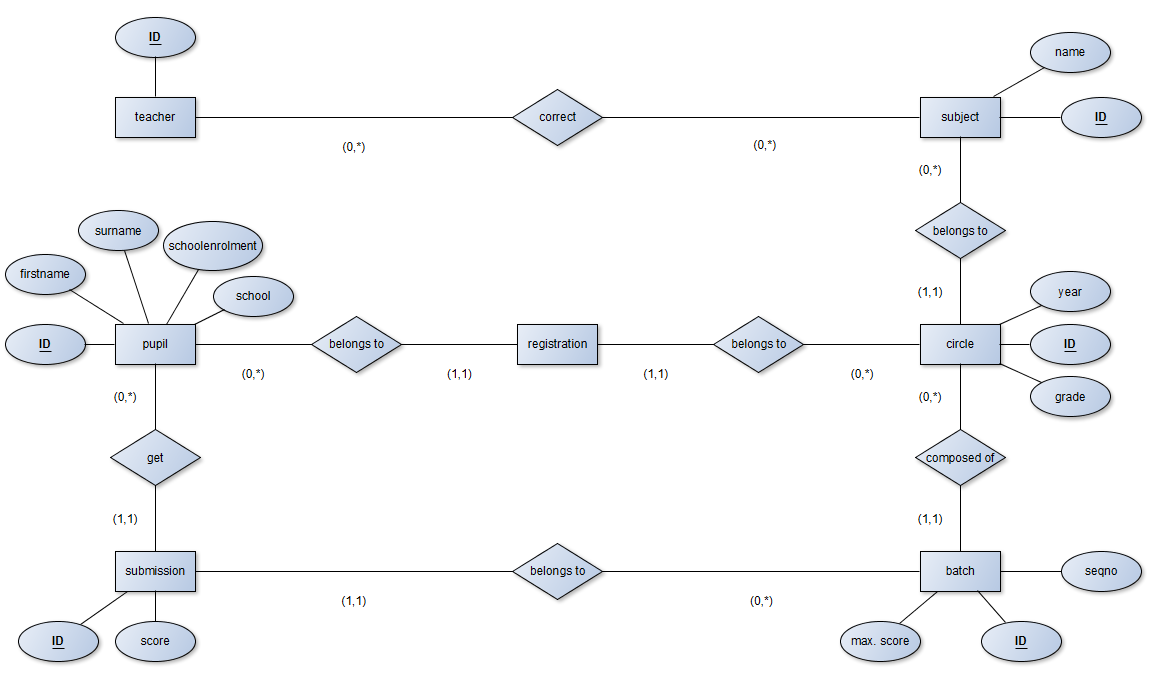
\includegraphics[scale=.55]{bilder/ER-Modell_engl.PNG}
	\caption{Beispielabbildung}
	\label{abb:beispiel}
\end{figure}
